\documentclass{article}
\usepackage{amsmath}
\usepackage{amssymb}
\usepackage{pgf}
\usepackage{tikz}
\usetikzlibrary{arrows,automata}
\usepackage[latin1]{inputenc}
\usepackage{lipsum}       % for sample text
\usepackage{changepage}   % for the adjustwidth environment

\title{Project 4}
\author{Jesse Adams, Dominic Orsi, Ben Puryear}
\date{September 28th, 2023}

\begin{document}

\maketitle

\section{Using the construction proof we developed to argue that the class of regular languages is closed under concatenation (Th. 1.47), draw an NFA that the recognizes the concatenation of the following languages:
 }
$\Sigma = \{0, 1\}$\\
$\text{Let } w \text{ be a string over } \Sigma$\\
$L1 = \{ w | \text{length of }w\text{ is at most } 5 \}$\\
$L2 = \{ w | \text{every odd position of }w\text{ is a } 1 \}$

\begin{center}
    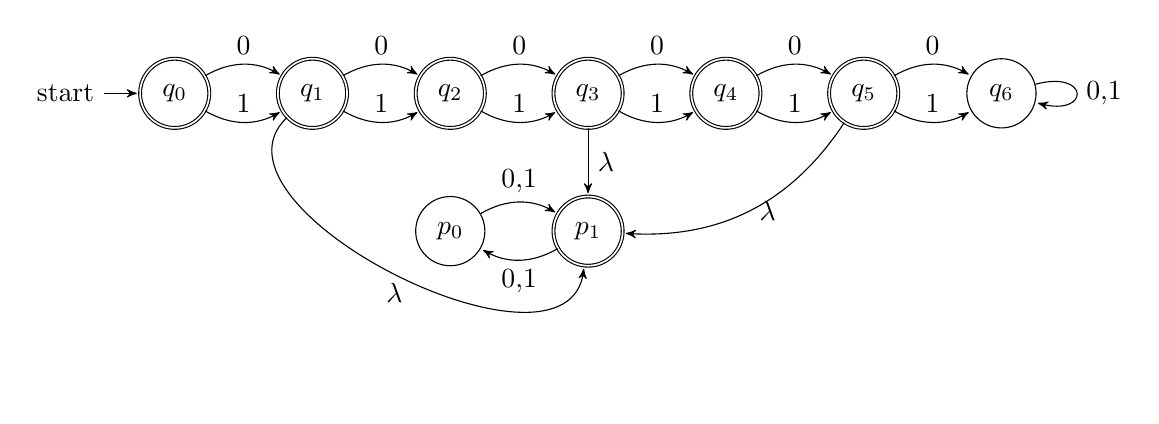
\begin{tikzpicture}[->,>=stealth',shorten >=1pt,auto,node distance=1.75cm]
        \tikzstyle{every state}=[fill=none,draw=black,text=black]
        \node[initial,double, state]  (0)                     {$q_0$};
        \node[double, state]  (1)            [right of=0]         {$q_1$};
        \node[state, double]  (2) [right of=1]  {$q_2$};
        \node[state, double]  (3) [right of=2]  {$q_3$};
        \node[state, double]  (4) [right of=3]  {$q_4$};
        \node[state, double]  (5) [right of=4]  {$q_5$};
        \node[state]  (6) [right of=5]  {$q_6$};

        \node[state] (10) [below of=2]{$p_0$};
        \node[state,double] (11) [right of=10] {$p_1$};

        \path (0) edge [bend left]   node            {0} (1)
        edge [bend right]                node            {1} (1)
        (1) edge [bend left]    node            {0} (2)
        edge [bend right]   node            {1} (2)
        edge [bend right=110] node[below] {$\lambda$} (11)
        (2) edge [bend left]               node    {0} (3)
        edge [bend right]    node            {1} (3)
        (3) edge [bend left]               node    {0} (4)
        edge [bend right]    node            {1} (4)
        edge  node[right] {$\lambda$} (11)
        (4) edge [bend left]               node    {0} (5)
        edge [bend right]    node            {1} (5)
        (5) edge [bend left]               node    {0} (6)
        edge [bend right]    node            {1} (6)
        edge [bend left] node[right] {$\lambda$} (11)
        (6) edge [loop right]               node    {0,1} (6)

        (10) edge [bend left] node {0,1} (11)
        (11) edge [bend left] node {0,1} (10);
    \end{tikzpicture}
\end{center}

\section{For regular languages, $A$ and $B$, the interleave of $A$, $A\_B$ is defined as follows:}

$A\_B = \{w | w = a_1 b_1 ... a_n b_n$ where $s_A = a_1 ... a_n \in A $ and $s_B = b_1 ... b_n \in B\}$
\\
That is, for each string $s_A$ in $A$ and $s_B$ in $B$, there is a string $s_{A\_B}$ in $A\_B$ whos elements are taken from $S_A$ and $S_B$ alternate and in order.
\\
\\
Use a construction to show that the class of regular languages is closed under interleaving.  A way to begin thinking about this is to define two machines, $M_A$ and $M_B$ that recognize languages $A$ and $B$.  Then design a machine $M_{A\_B}$ that alternates between the states of $M_A$ and $M_B$ as it reads an interleaved string.
\\
\\
To get started, design two simple machines, one that accepts an even number of 0s over $\{0,1\}$, the other that accepts an even number of $X$s over $\{X,Y\}$. Then the states of $M$ the machine that accepts the interleaved strings of the two machines are 3-tuples, $Q_A \times Q_A \times \{1,2\}$ where $1$ in the 3rd position indicates that $M_A$ runs and and a $2$ in the in the 3rd position indicates that $M_B$ runs. The trick is in defining the transition functions.

\section{Here is an NFA. Using construction, convert the NFA to an equivalent DFA.}

\begin{center}
    \begin{tikzpicture}[->,>=stealth',shorten >=1pt,auto,node distance=3.75cm]
        \tikzstyle{every state}=[fill=none,draw=black,text=black]
        \node[state]  (1)            [right of=0]         {$1$};
        \node[state, double]  (2) [right of=1]  {$2$};
        \node[state]  (3) [below right of=1]  {$3$};

        \path (1) edge     node            {$a$} (3)
        edge [bend left]   node            {$\lambda$} (2)
        (2) edge                node    {$a$} (1)
        (3) edge [loop below]               node    {$b$} (3)
        edge     node            {$a,b$} (2);
    \end{tikzpicture}
\end{center}

\subsection{What is the full formal definition of the DFA?}

\subsection{What is the state transition diagram of the DFA.}

\begin{center}
    \begin{tikzpicture}[->,>=stealth',shorten >=1pt,auto,node distance=3.75cm]
        \tikzstyle{every state}=[fill=none,draw=black,text=black]
        \node[state]  (1)            [right of=0]         {$\theta$};
        \node[state, double]  (2) [right of=1]  {$1,2$};
        \node[state]  (3) [below of=1]  {$2,3$};
        \node[state]  (4) [right of=3]  {$1,2,3$};

        \path (1) edge     node            {$a$} (3)
        edge [bend left]   node            {$\lambda$} (2)
        (2) edge                node    {$a$} (1)
        (3) edge [loop below]               node    {$b$} (3)
        edge     node            {$a,b$} (2);
    \end{tikzpicture}
\end{center}

\end{document}